\chapter{Feature-based approach}
\label{cha:FeatureApproach}

To solve the main drawbacks of finding reliable point correspondences for an initial alignment of $C_1$ and $C_2$ the focus on the second approach lies on point features. They are introduced as they provide additional, meaningful information about a point $\boldsymbol{p}_i$ besides its coordinates. For this reason, point feature histograms, namely ``Fast point feature histograms'' (FPFH) \cite{FPFH} are computed for all points of $C_1$ and $C_2$. Basically, a histogram of a point $\boldsymbol{p}$ describes the curvature of a surface described by itself and its $k$ neighbors. By detecting similar point feature histograms between $C_1$ and $C_2$, referred to as feature matching, point correspondences are acquired. These are then used for an initial alignment of $C_1$ and $C_2$ that their largest rigid parts overlap. Proceeding from the largest rigid part, linked rigid parts can be detected. This approach is closely related to Guo et al \cite{guo2016correspondence}. 

\section{Fast point feature histograms}
\label{FPFH}
The ``Fast Point Feature histograms'' algorithm is an improved approach of the `'Persistent Point Feature Histogram for 3D Point Clouds'' \cite{PPFH} in terms of computation time. It focuses on computing a feature histogram for a point $\boldsymbol{p}$ by comparing its normal $\vec{n}$ to the normals of all $k$ neighbors. The choice of those point features are the following: 
%%
\begin{itemize}
	\item rotation- and scale-invariant
	\item easy comparison of feature histograms
	\item approval of approach
	\item straightforward adaption of different dimensions (2D and 3D)
\end{itemize}
%%
The data input for this algorithm is a list of $n$ unordered points $\boldsymbol{p}_1(x,y,z), \cdots, \boldsymbol{p}_n(x,y,z)$ only providing information about the points coordinates in 3D space. As a result, no surface is supplied for the computation of feature histograms. Therefore, in an initial step the point normals need to be computed (see subsection \ref{normal}).

\subsection{Normal estimation}
\label{normal}
As a first step, the normals of all unordered points from the input clusters $C_1$ and $C_2$ are estimated, following the approach of Hoppe et al \cite{normals}. The normal $\vec{n}$ of point $\boldsymbol{p}$ can be computed by taking all neighboring points $k$ within a radius $r$ of $\boldsymbol{p}$ into consideration. Subsequently, a least error fit straight line $X$ in the form $ax + by +c = 0$ to all selected points including $\boldsymbol{p_i}$ is computed by minimizing the squared distances from all points
%%
\begin{equation}
\begin{split}
dist^2(x_i, y_i) = (ax_i + by_i + c)^2
\\
e =   \displaystyle\sum_{i=1}^{k} dist^2(x_i, y_i)
\end{split}
\end{equation}
%%
to $X$. This is done by computing the unknown parameters $a, b$ of $X$ with the covariance matrix 
%%
\begin{equation}
\begin{pmatrix}
\overline{x^2} - \overline{x} \cdot \overline{x} & \overline{xy} -\overline{x} \cdot \overline{y}\\
\overline{xy} -\overline{y} \cdot \overline{x} & \overline{y^2} -\overline{y} \cdot \overline{y}
\end{pmatrix} \cdot \begin{pmatrix}
a \\
b
\end{pmatrix} = \lambda \cdot \begin{pmatrix}
a \\
b
\end{pmatrix}
\end{equation}
%%
resulting in two pairs of an eigenvalue and eigenvector $(n_1,\lambda_1)$ and $(n_2,\lambda_2)$. The normal of $\boldsymbol{p}$ is computed solving the linear equation for the normal vector $\vec{n_2}$ which is represented by $\lambda_2$. The procedure is conducted for all points from $C_1$ and $C_2$ (see figure \ref{fig:normalEstimation}). 
%%
\begin{figure}[H]
	\centering
	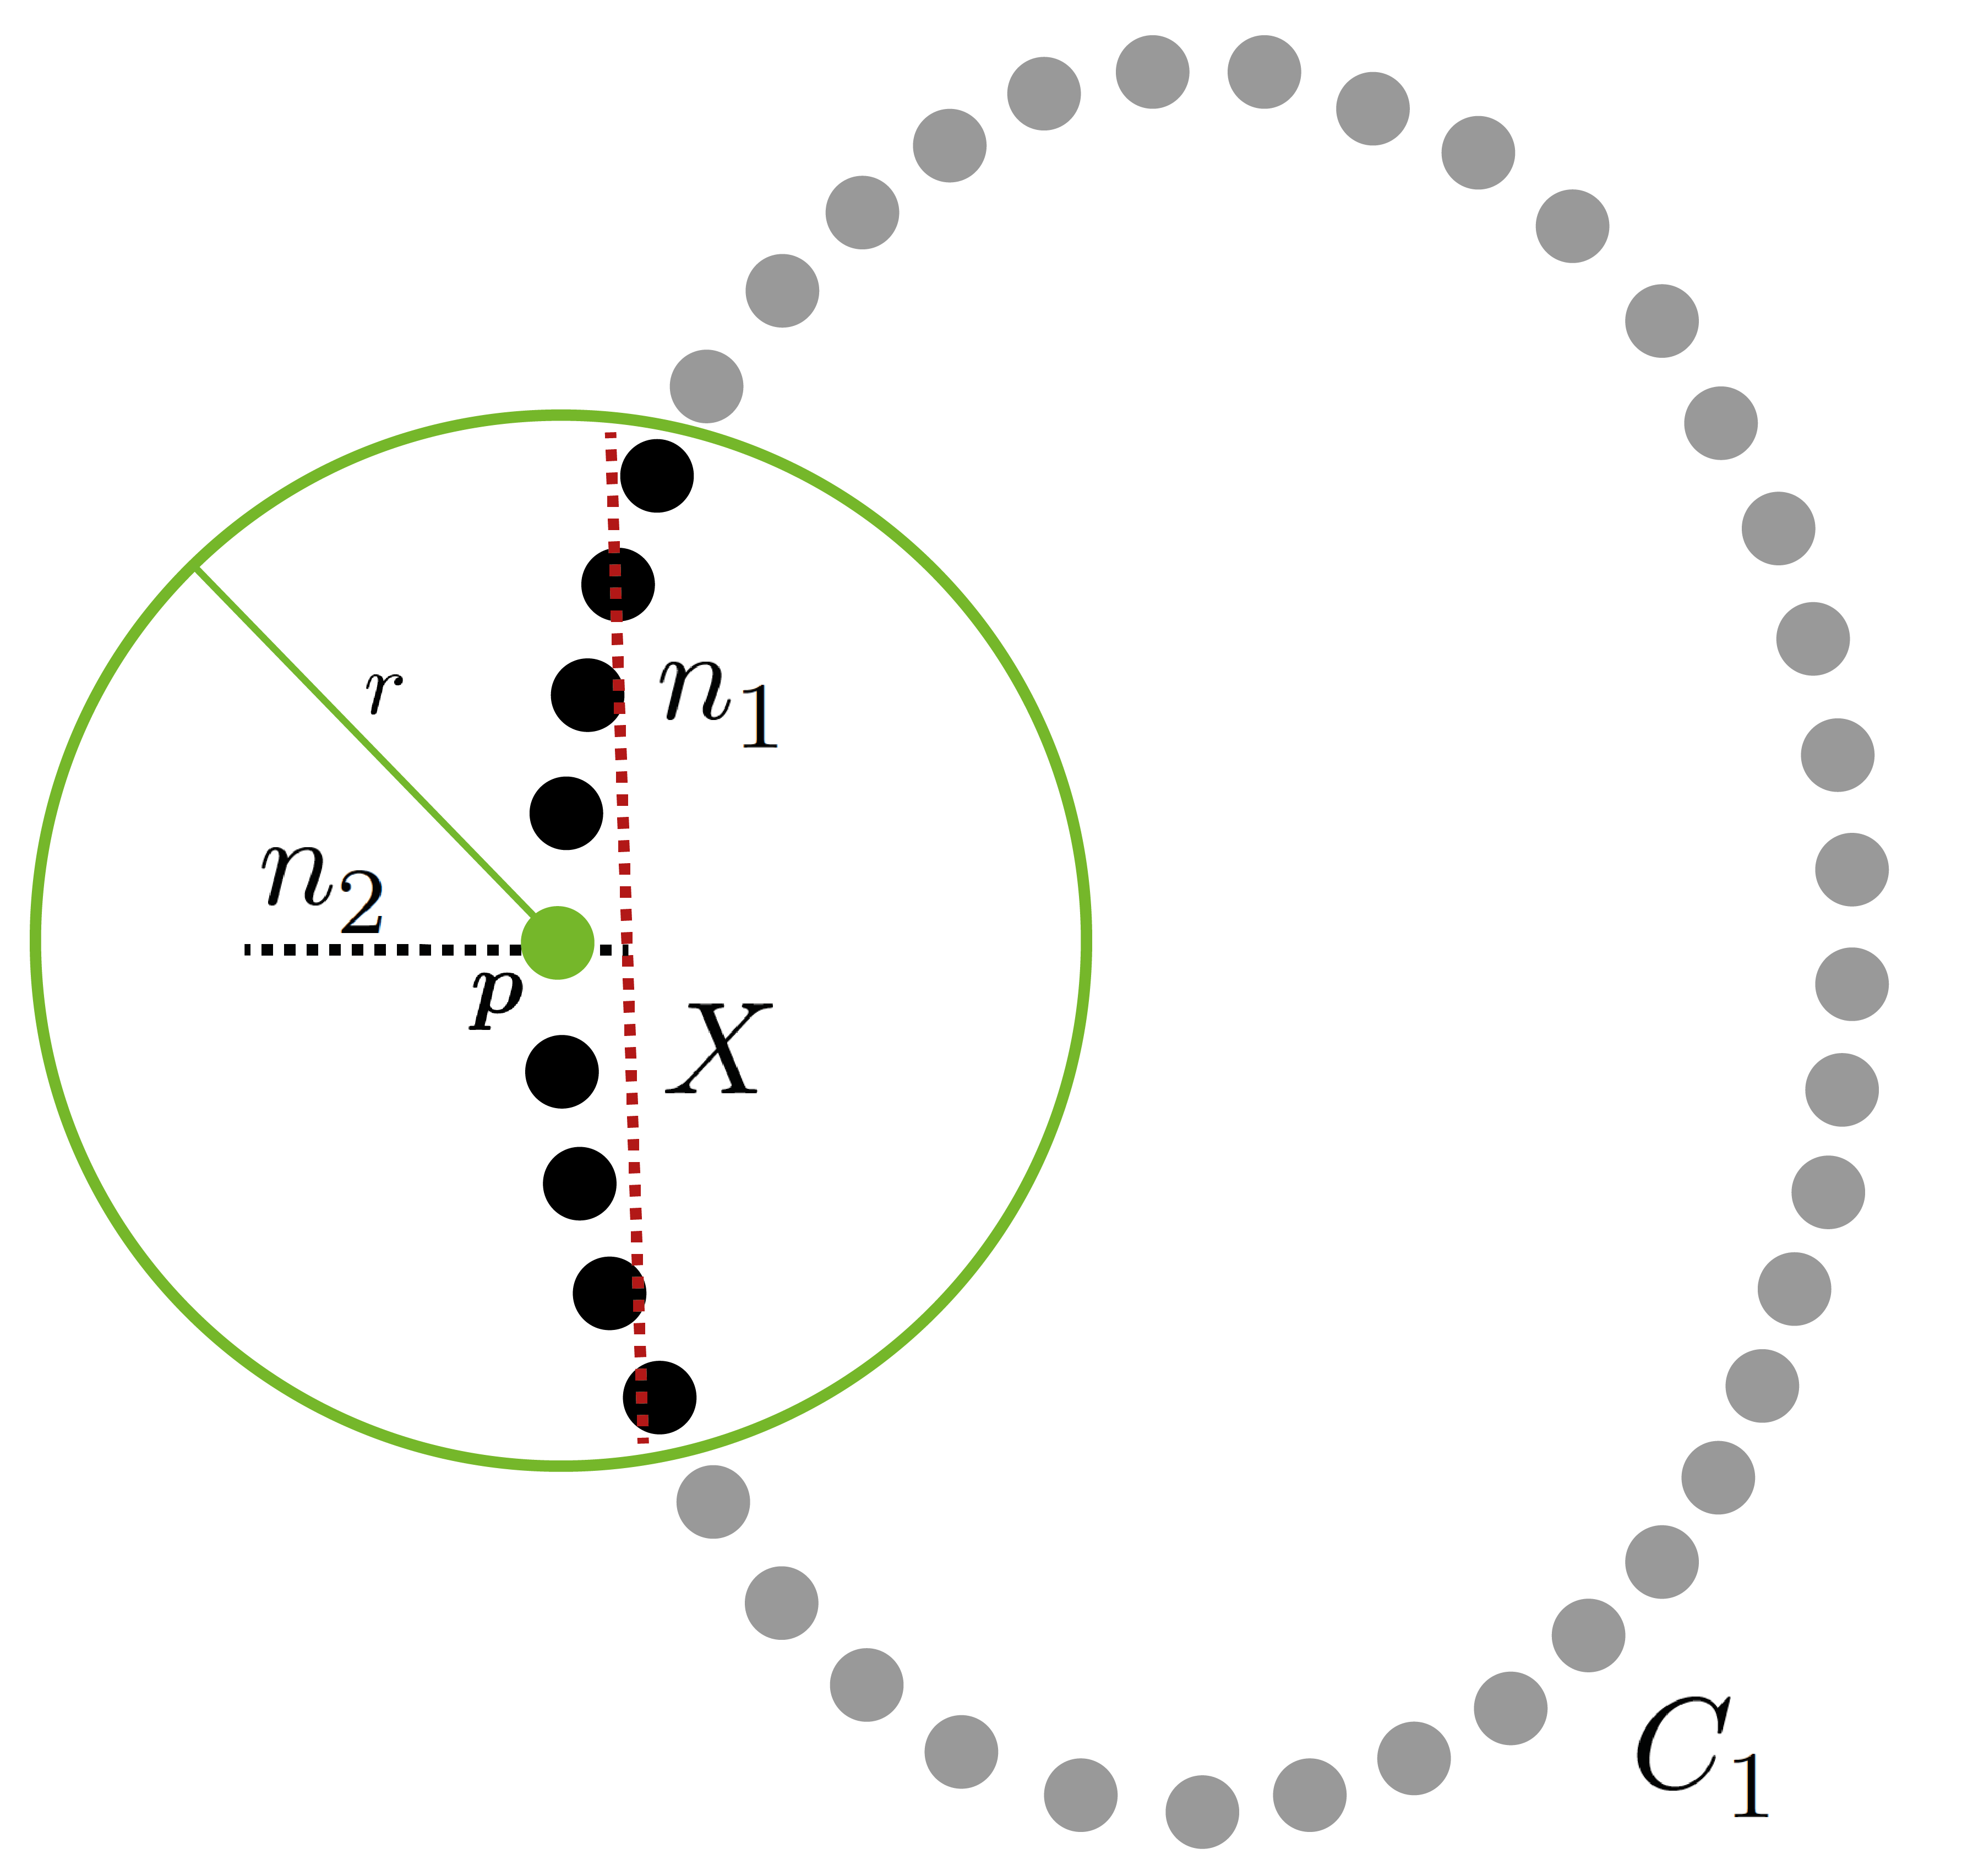
\includegraphics[width=0.4\linewidth]{normalEstimation}
	\caption{Normal estimation for a cluster point $\boldsymbol{p}$ of $C_i$ by a computation of the least squared fitting line $X$ of the neighborhood inside a radius $r$. Calculation of the eigenvectors $\vec{n_1}$ and $\vec{n_2}$ by forming the covariance matrix of  $\boldsymbol{p}_i$ and all $k$ points.}
	\label{fig:normalEstimation}
\end{figure}
%%
%TODO: fix image (C_i, ...)
%%
As a next step, it is required that all normals are equally oriented, as some might be flipped by 180°. Basically, all $n$ computed normals are traversed globally, starting with a normal $\vec{n}$ of a point $p$. Thereby, it is of particular importance to select a normal that assures consistent orientations between $C_1$ and $C_2$. Taking its orientation as parent normal $\vec{n_p}$, the angle $\delta$ between $\vec{n_p}$ and all neighboring normals $\vec{n_k}$ 
%%
\begin{equation}
\delta = \vec{n_p} \cdot \vec{n_k}, \quad \text{for $|\vec{n_p}|, |\vec{n_k}| = 1$}
\end{equation}
%%
is computed. In case of $\delta < 0$, $\vec{n_k}$ requires to be flipped 180° ($\vec{n_k} = -\vec{n_k})$. If all $k$ normals have been verified to be oriented in consideration of $\vec{n_p}$ any $\vec{n_k}$ is selected as current $\vec{n_p}$. The whole algorithm proceeds until all $n$ normals have been verified to correspond with their parent normal $n_p$ (see figure \ref{fig:flipping}).
%%
%TODO: add image normal flipping
%%
\begin{figure}[H]
	\centering\small
	\begin{tabular}{cc}
		\fbox{
\includegraphics[width=0.40\textwidth]{Placeholder}} &	
		\fbox{
\includegraphics[width=0.40\textwidth]{Placeholder}} 
		\\
		(a) & (b) 
	\end{tabular}
	\caption{Normal flipping of all normals computed on a cluster $C_i$ (a) to equally orient them (b).} 
	\label{fig:flipping}
\end{figure}
%%
\subsection{SPFH and FPFH}
As an intermediate step before computing the FPFH, the simplified point feature histogram (SPFH) of a point $\boldsymbol{p}$ is computed, which represents its relationship to its $k$ neighbors. This is achieved by calculating three geometric features between $\boldsymbol{p}$ and each of its $k$ neighbors $\boldsymbol{p_k}$. For further calculations, $\boldsymbol{p}_i$ represents the point having the smaller angle between its normal and the line connecting the point set, $\boldsymbol{p}_j$ corresponds to the other point. Using their normals $n_i$ and $n_j$ a Darboux $uvn$ frame $(u = n_i, v = (p_j - p_i) \times u, w = u \times v)$ is computed. Consequently, the following angles
%%
\begin{equation}
\begin{split}
\alpha = v \cdot n_j
\\
\phi = (u \cdot (p_j - p_i))/\|p_j - p_j\|
\\
\theta = arctan(w \cdot n_j, u \cdot n_j)
\end{split}
\label{eq:AngularVariations}
\end{equation}
%%
are computed which are categorized into a histogram (see subsection \ref{histogram}). The SPFH of $\boldsymbol{p}$ is then weighted to its FPFH
%%
\begin{equation}
FPFH(\boldsymbol{p}) = SPF(\boldsymbol{p}) + \frac{1}{n} \cdot \displaystyle\sum_{k=1}^{n}\frac{1}{w_k} \cdot SPF(p_k)
\end{equation}
%%
by computing the SPFH for all of its $k$ neighbors. The weight $w_i$ represents the distance $d(\boldsymbol{p},\boldsymbol{p}_k)$. The influence region diagram for a Fast Point feature histogram of a query point $\boldsymbol{p_q}$ can be seen on Figure \ref{fig:FPFHregion}. 
%%
\begin{figure}[H]
	\centering
	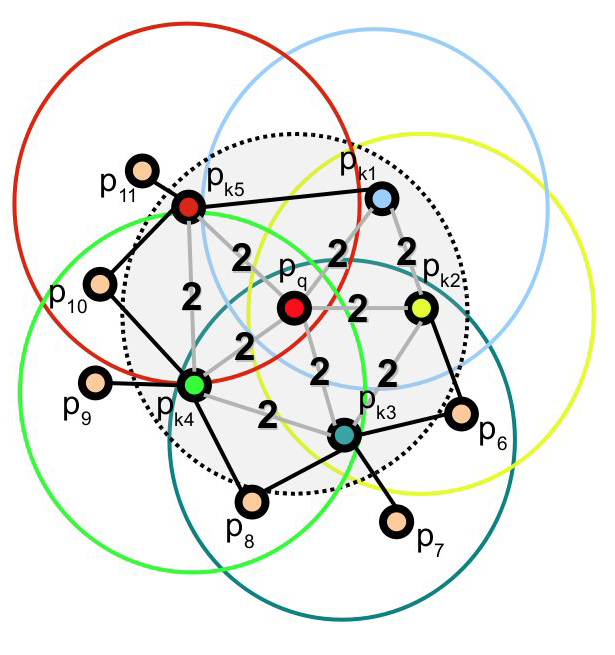
\includegraphics[width=0.4\linewidth]{FPFH_region}
	\caption{The point region for the calculation of the feature histogram for a query point $\boldsymbol{p}_q$. The SPFH of $\boldsymbol{p}_q$ and its neighbors (inside the grey circle) is weighted with the SPFHs of all $k$ neighbors (colored circles) \cite{FPFH}.}
	\label{fig:FPFHregion}
\end{figure}
%%
\subsection{Feature histograms}
\label{histogram}
The resulting feature values for each point $p$ of $C_1$ and $C_2$ in form of three angles between its neighbors $k$ are categorized using a histogram $H \{bin_1,\ldots,bin_b\}$ with $b = q^f$ bins to consider all possible combinations of the feature values. Thereby, $q$ represents the number of intervals the feature values should be categorized into. The number of feature values is represented by $f$, in this case three. Taking into account three feature values computed between a point set ($p$,$p_k$) the associated bin at the index $idx$
%%
\begin{equation}
idx = \displaystyle\sum_{i=1}^{i \leq f}q(f_i) \cdot 2^{i-1}
\end{equation}
%%
is incremented by 1. The function $q(f)$ returns the interval the feature is allocated to, ranging from 0 to $q - 1$. Finally, each bin contains the number of point pairs that are allocated in the specified value interval.As soon as the feature histograms of all points from $C_1$ and $C_2$ are computed only salient histograms are taken as comparison for point correspondence between $C_1$ and $C_2$ to reduce the correspondence space. In order to achieve that, the mean of all feature histograms $\mu$ of a cluster $C_i$ is computed. Subsequently, the distance of a feature histogram $H_i$ is compared to $H_\mu$ and in case of being outside the value $\mu \pm \sigma$ denoted as \textit{unique} and passed to the next step of detecting matching histograms between $C_1$ and $C_2$. The standard deviation
%%
\begin{equation}
\sigma = \frac{1}{N} \cdot \displaystyle\sum_{i=1}^{N}(H_i(b) - \overline{H_i})^2
\end{equation}
%%
is therefore calculated for all histograms $H_i$ with $N$ data entries of all cluster points. 
%%
\subsection{Feature matching}
\label{histogramCriteria}
As a next step, all \textit{unique} feature histograms of $C_1$ are aiming for detecting the most similar feature histogram from $C_2$. For that reason, different histogram-similarity criteria have to be determined to measure the similarity between two histograms $H_j$ and $H_k$ with each $b$ bins. In order to detect the best fitting histogram three main criteria most frequently applied in reference papers \cite{surfletPairRelation} \cite{localFeatureHistograms} are selected. As first criterion the squared euclidean distance (L2)
%%
\begin{equation}
\varepsilon(H_j, H_k) = \displaystyle\sum_{i=1}^{b}(H_j(i) - H_k(i))^2
\end{equation}
%%
is computed. In the reference paper of Guo et al. \cite{guo2016correspondence} the euclidean distance was selected as similarity criterion between feature histograms. It generally generates more point correspondences (see section \ref{ResultsLRP}) than the other two criteria. Furthermore, the statistical Chi-Square ($\chi^2$) divergence
%%
\begin{equation}
\chi^2(H_j, H_k) = \displaystyle\sum_{i=1}^{b}\frac{(H_j(i) - H_k(i))^2}{(H_j(i) + H_k(i))}
\end{equation}
%%
is examined which achieves less point correspondences than the L2 form but with a higher success rate. Finally, the Kullback-Leibler (KL) divergence
%%
\begin{equation}
\kappa(H_j, H_k) = \displaystyle\sum_{i=1}^{b}(H_j(i) - H_k(i)) \cdot ln \frac{H_j(i)}{H_k(i)}
\end{equation}
%%
is calculated, which is the most computational expensive one due to the application of $ln$. As a histogram with $q^f$ bins might contain a lot of zero values, in case of a division or logarithm all zero-values are replaced by the value 1.

\subsection{Adaptions for 2D}
\label{adaptions}
In order to compute the proposed feature histograms for 2D points, these need be treated like 3D points. This is achieved by setting each z-coordinate to 0 to allow all calculations originally targeting 3D points. 
2D point clouds are generally composed of less points than 3D point cloud, which results in less neighbor points for normal estimation and feature computation. As a result the computation time can be considerable reduced. 
As also the number of point correspondences are considerable reduced, all histograms are considered during the feature histogram matching, not only salient ones. 

\section{LRP algorithm}
\label{LRP}
The approach from Guo et al \cite{guo2016correspondence} aims to detect the largest rigid part (LRP) of two poses of an object to have a solid basis for a successful segmentation into the rigid parts. A similar procedure is aspired after in the proposed feature-based approach.

\subsection{Basic functionality}
\label{functionalityLRP}
As an initial step, the LRP algorithm attempts to detect the most reliable correspondences between two clusters $C_1$ and $C_2$. For that, local point descriptors (see section \ref{FPFH}) are computed. The requirement for a sparse correspondence between two cluster points $\boldsymbol{p}_i(x,y)$ and $\boldsymbol{p}_j(x,y)$ is that they are \textit{reciprocal}, which means that the according point feature histograms are the most similar from each other. Some of the sparse correspondences are assumed to be wrong. Therefore, RANSAC is applied on the point correspondences to aim for a single rigid transformation to detect the so-called ``largest rigid part'' (LRP), which is supported by the largest corresponding point cluster between $C_1$ and $C_2$. In case of a human, this would be the torso. Subsequently, all linked rigid parts to the LRP are detected by recursively applying the algorithm on grown clusters from the current LRP.

\subsection{Input data}
For the proposed 2D implementation, the 2D hulls of an articulated object in two different poses are taken as input (see Figure \ref{fig:inputPoses}). To support the point cohesiveness of a rigid parts after a transformation or segmentation joint-likely spheres were placed between rigid parts which are also used as rotation points. For the computation, those are treated to belong to a rigid part and no information about a joint are extracted. To achieve an indicator for the adjustment of thresholds (e.g. maximum distance to closest point), the resolution of the input clusters is computed. By applying the approach from \ref{clustering} the estimated resolutions accounts to 7.24 for $C_1$ and 7.56 for $C_2$.
%%
\begin{figure}[H]
	\centering\small
	\begin{tabular}{cc}
		\fbox{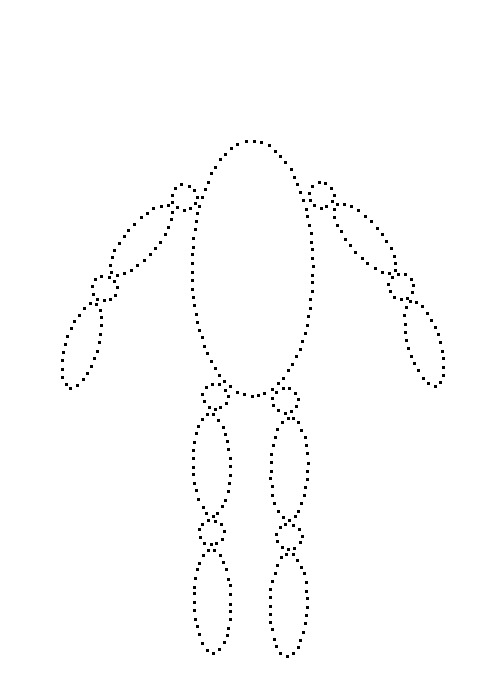
\includegraphics[width=0.40\textwidth]{InputPose1}} &	
		\fbox{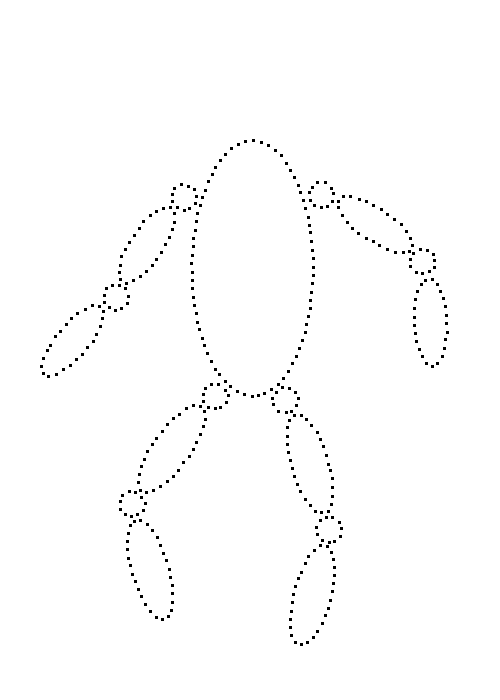
\includegraphics[width=0.40\textwidth]{InputPose2}} 
		\\
		(a) & (b) 
	\end{tabular}
	\caption{Taking an articulated object (puppet) in two different poses $C_1$ (a) and $C_2$ (b) in form of a 2D point cloud representing its hull as input.} 
	\label{fig:inputPoses}
\end{figure}
%%
\subsection{Implementation steps}
In order to re-implement the algorithm in 2D, only minor modifications concerning point coordinates and feature histograms had to be accomplished (see subsection \ref{adaptions}). The most crucial part of the whole algorithm is the initial alignment of $C_1$ and $C_2$ in order to detect the actual largest rigid part of the articulated object. This step is of particular importance, as the subsequent detection of further rigid parts proceeds from there. Concerning the detection of linked rigid parts, an approach with less computation steps and time was implemented. Generally, the implementation can be split into main parts.
\begin{enumerate}
	\item The PCA is employed on the input clusters $C_1$ and $C_2$ to estimate the normals of all points.
	\item Point feature histograms (FPFH) are computed for all points of $C_1$ and $C_2$. Sparse point correspondences are computed by feature matching. A point correspondence needs to be \textit{reciprocal}.
	\item The RANSAC approach is applied on these correspondences to detect a transformation $T$ that aligns $C_1$ and $C_2$. In each iteration, clusters are detected from overlapping points. The LRP is assigned to the resulting biggest point cluster.
	\item Unmatched clusters from $C_1$ and $C_2$ are taken as input to detect linked rigid parts from the LRP, which is achieved by region growing.
	\item Joints are estimated between the current LRP an all detected clusters linked to the LRP. Those are considered for allocating corresponding rigid parts of $C_1$ and $C_2$.
	\item Linked rigid parts are detected by rotating a cluster around its joint and finding the largest overlapping cluster. Certain constraints and a weighted error are taken into account.
\end{enumerate}

\subsection{Detection of sparse correspondences}
\label{correspondences}
As a first, the normals as well as the feature histograms for all points of $C_1$ and $C_2$ (see section \ref{FPFH}) are computed. Results of the normal flipping procedure can be seen on figure \ref{fig:normalFlipping}.

%TODO: Picture of normal flipping
\begin{figure}[H]
	\centering\small
	\begin{tabular}{cccc}
		\fbox{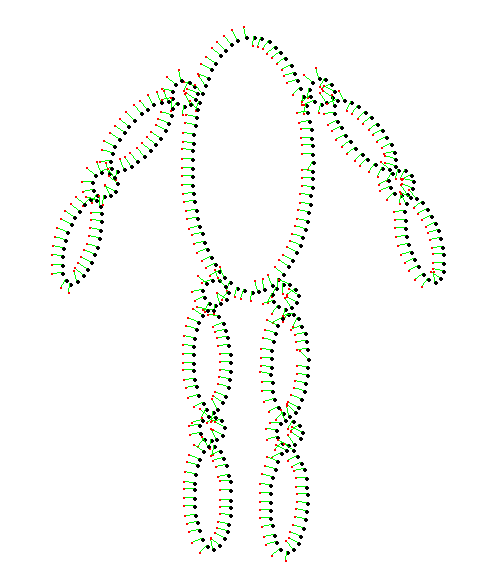
\includegraphics[width=0.23\textwidth]{Normals_C1_cropped}} &	
		\fbox{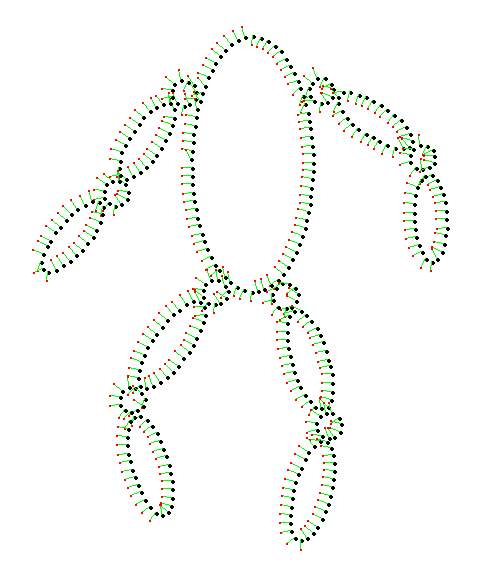
\includegraphics[width=0.23\textwidth]{Normals_C2_cropped}} &	
		\fbox{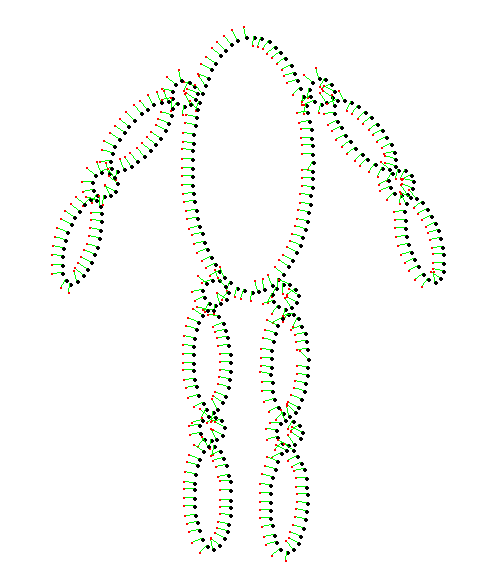
\includegraphics[width=0.23\textwidth]{Normals_C1_cropped}} &	
		\fbox{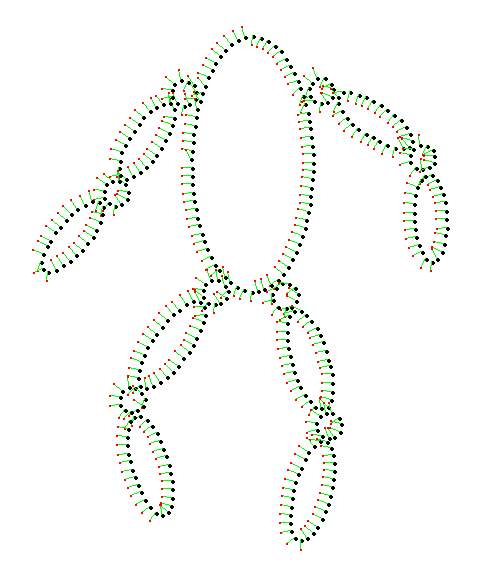
\includegraphics[width=0.23\textwidth]{Normals_C2_cropped}} 
		\\
		(a) & (b) & (c) & (d)
	\end{tabular}
	\caption{Normal estimation of two Cluster $C_1$ and $C_2$ (a) and (b) a subsequent global traversing of all normals to orient them similar (c) and (d).} 
	\label{fig:normalFlipping}
\end{figure}
It can be observed that the flipping of normals does not globally succeed. The causes are corner positions of the 2D hull. Considering two normals surrounding a corner point, the normals are expected to face each other. But during the normal flipping they are similarly oriented, although the corner point between them should counteract this behavior. For this reason the global flipping of the normals, considering the given data set, leads to a high number of false point correspondences. A possible solution would be the introduction of more points, especially forming a corner.
%%
%TODO: test with new dataset
%%
For the detection of sparse correspondences between $C_1$ and $C_2$ three histogram distances (see section \ref{histogramCriteria}) are taken into account. Depending on the chosen distance as criteria, more or less correspondences can be detected, refer to section \ref{ResultsLRP} for a detailed comparison. The mean histogram of all histograms as well as a \textit{unique} histogram can be seen on \ref{fig:meanHistogram}. 
%%
%TODO: Picture of mean histogram + similar histogram
%%
\begin{figure}[H]
	\centering\small
	\begin{tabular}{cc}
		\fbox{
\includegraphics[width=0.45\textwidth]{Placeholder}} &	
		\fbox{
\includegraphics[width=0.45\textwidth]{Placeholder}} 
		\\
		(a) & (b) 
	\end{tabular}
	\caption{Computing the $\mu$ histogram of $C_1$ to represent frequently arising feature histograms (a). A \textit{unique}  histogram is stated by considerably deviating from the $\mu$ histogram (b).} 
	\label{fig:meanHistogram}
\end{figure}
Figure \ref{fig:sparseCorrespondences} represents the point correspondences between $C_1$ and $C_2$ resulting from feature matching. It is clearly evident that points located near a corner are more likely to detect a reciprocal point correspondence than points located at smooth surfaces. The reason is, that those features are determined as \textit{unique} which makes them more distinguishable. On the contrary, all points located on a smooth surface have similar feature histograms.
%%
\begin{figure}[H]
	\centering \small
	\begin{tabular}{c}
		\fbox{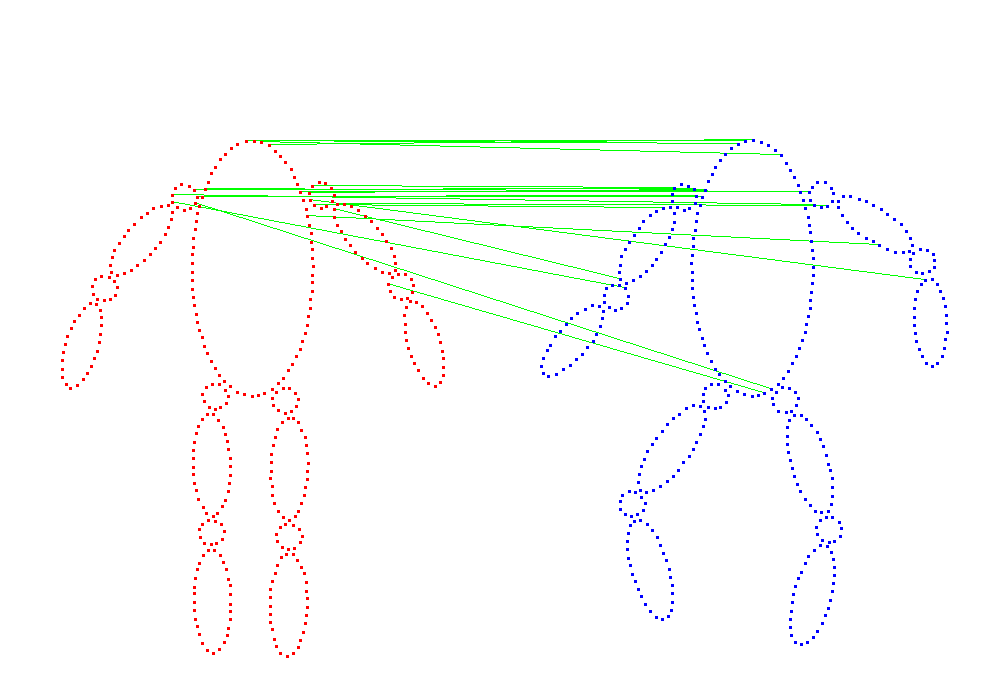
\includegraphics[width=0.80\textwidth]{featureCorrespondences_chiSquare}} 
	\end{tabular}
	\caption{Visualization of the point correspondences established from most similar, reciprocal feature histograms using the chi-square distance between all points of $C_1$ (red) and $C_2$ (blue).}
	\label{fig:sparseCorrespondences}
\end{figure}
%%
As some of those correspondences are assumed to be wrong, a RANSAC approach is applied on all correspondences to reject false ones (see subsection \ref{detectionLRP}).
%%
\subsection{Detection of the largest rigid part}
\label{detectionLRP}
The dense point correspondences from the previous computation step (see subsection \ref{correspondences}) may contain several errors. Therefore, RANSAC is applied as a next step to detect a single rigid transformation $T$ that leads to the biggest overlapping point cluster of $C_i$ and $C_j$. Thereby, in each iteration, 2 random correspondences are selected and used for the calculation of $T$ which is applied on $C_i$ to be translated on $C_j$. 
%%
%TODO: Show Matrices of the RANSAC
%%
The number of iterations highly depends on the ratio of right and wrong point correspondences. Based on visual assessments and the calculated probability of a choosing two correct correspondences
%%
%TODO: number of iterations? --> number of false correspondences, formular
%%
the number of iterations is set to 500.
%%
In each iteration, clusters are grown from all overlapping points with an euclidean distance $d(\boldsymbol{p}_i,\boldsymbol{p}_j)$ again below a predefined threshold $\tau$. The procedure is applied both on $C_i$ and $C_j$ which results in two rigid parts as output representing the largest detected clusters (see figure \ref{RANSAC}).
%%
\begin{figure}[H]
	\centering\small
	\begin{tabular}{cc}
		\fbox{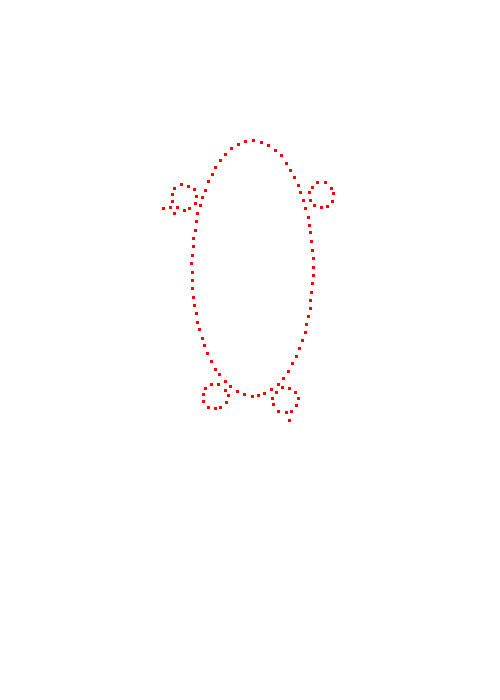
\includegraphics[width=0.40\textwidth]{RANSAC_1000_chiSquare_ref}} &	
		\fbox{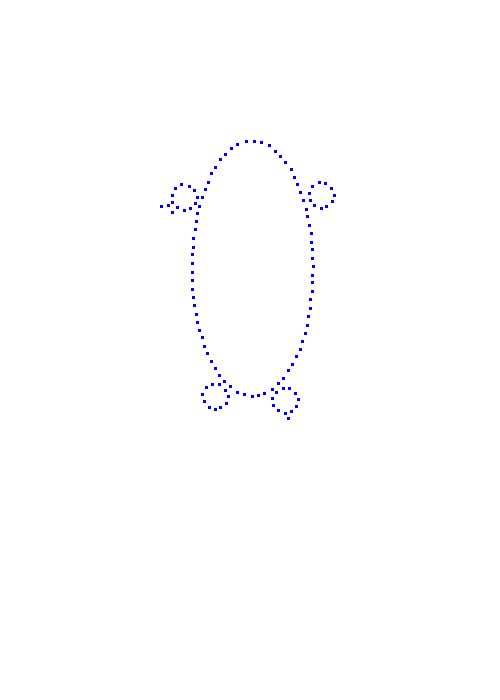
\includegraphics[width=0.40\textwidth]{RANSAC_1000_chiSquare_target}} 
		\\
		(a) & (b) 
	\end{tabular}
	\caption{Computation of the largest rigid part from $C_1$ (a) and $C_2$ (b) by applying RANSAC on the detected point correspondences.} 
	\label{fig:RANSAC}
\end{figure}
%%
The final transformation $T$ of the RANSAC approach, which leads to the largest overlapping clusters, is applied on the reference cluster. This procedure is required in order to similarly align $C_1$ and $C_2$ for further computations (see subsection \ref{CorrespondingClusters}).

\subsection{Cluster detection by region growing}
\label{cluster}
After successfully detecting a ``largest rigid part'' $P_i$ and $P_j$ for each input clusters $C_i$ and $C_j$ they are added to a list of rigid parts $\mathcal{P}$. Potential linked rigid parts are detected from region growing of all unclustered points $\mathcal{U} =  \{\boldsymbol{u}_1,\ldots,\boldsymbol{u}_n\}$. Those comprise all cluster points of $C_1$ and $C_2$ excluding already detected largest rigid parts $\mathcal{P}$. An adapted region growing procedure from subsection \ref{RegionGrowing} is applied with the previously detected LRP as seed. 
For this approach, it does not only return the largest cluster, but all clusters above a certain size. The result is a set of clusters $\mathcal{C}$ for each $C_i$ and $C_j$. As a next step, a preliminary joint $\boldsymbol{j}$ is estimated for each output clusters. This is achieved by detecting the closest points between $P_i$ and one of its clusters $C_i$. The joints are required for the detection of corresponding cluster between $C_1$ and $C_2$ (see subsection \ref{CorrespondingClusters}). Furthermore, there are used as joint weights for the detection of linked rigid parts (see subsection  and \ref{JointWeights}).

\subsubsection{Establishment of corresponding clusters}
\label{CorrespondingClusters}
In case of detecting more than one cluster resulting from region growing from each $P_1$ and $P_2$ it must be verified which clusters correspond to each other. This might be for example the case for the extremities linked to the torso. This association step is essential, as the detection of linked parts to the previously detected LRP assumes two clusters representing the same set of rigid parts. Thereby, the provisional joints $\mathcal{J}$ estimated for all clusters are used to associate two clusters of $C_1$ and $C_2$. Thereby the clusters with reciprocal closest joints, represented by the euclidean distance $d(\boldsymbol{j}_i,\boldsymbol{j}_j)$, are assumed as associated clusters.

\subsection{Detection of linked rigid parts}
\label{JointWeights}
In the reference paper the feature matching in combination with RANSAC for detecting point correspondences was reapplied on the linked clusters to the already detected rigid parts. However, this approach is not successful in the current 2D application. The reason is that the point features are not meaningful due to the reduced number of points and similarity of shapes. In order to iteratively detect further rigid parts linked to already detected ones another approach is developed which manages to operate less computational-expensive and less time-consuming as RANSAC and feature computation is not required. Thereby, the knowledge is used that rigid parts are transformed by rotating around a joint. For that purpose, the estimated joints $\mathcal{J} = j_1,\cdots,j_n$ resulting from the approach of subsection \ref{cluster} are taken into account. As a first step, two input clusters $C_i$ and $C_j$ are transformed that their joints overlap. Next, the primary axis of $C_i$ and $C_j$ are aligned to guess an initial alignment which should further reduce the computation steps. Then, $C_i$ is iteratively rotated around its joint into the direction of an decreasing least squares error $e$ in order to overlap with $C_j$. By iteratively updating $e$ after each rotation step, a best overlapping position between the linked rigid parts can be detected. Thereby, the preliminary joints are used as weights. A point $p_i$ being located far away from its allocated joint $J_n$ does not contribute as much to the matching error as points located near the joint. A weight $w$ is calculated by comparing the distance $d(p_i, J_n)$ to the maximal distance $d_{max}$ between $J_n$ and the farthermost allocated point. Subsequently a total matching error $e$
%
\begin{equation}
\begin{split}
w_i = \| \boldsymbol{p}_i - \boldsymbol{j}_n\| \cdot \frac{1}{d_{max}}
\\
e = \displaystyle\sum_{i=1}^{m}\| \boldsymbol{p}_i - \boldsymbol{q}_i\|^2 \cdot (1 - {w_i})^2
\end{split}
\label{eq:jointWeightError}
\end{equation}
%
is achieved by combining the distance of a point to its closest point and the joint weight $w$. The error is squared in order to further weaken the influence of cluster points being located far away from the joint. The final detected rigid parts are represented by the biggest cluster resulting from a rotation with the lowest error $e$. As a last step, all points with a closest point below a certain threshold $\tau$ are taken as input for region growing. It is assumed, that two linked rigid parts are quite similar aligned, therefore the distance threshold $\tau$ is considerable small. The largest cluster is finally returned as detected linked part.
%%
\begin{figure}[H]
	\centering\small
	\begin{tabular}{ccc}
		\fbox{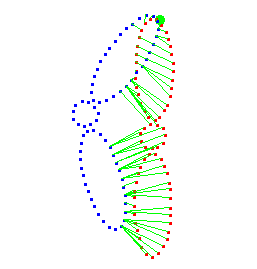
\includegraphics[width=0.30\textwidth]{LegRotation_Before_cropped}} &	
		\fbox{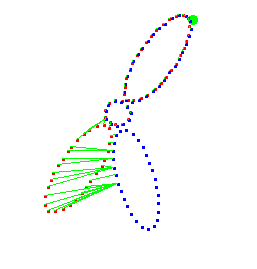
\includegraphics[width=0.30\textwidth]{LegRotation_After_cropped}}  &	
		\fbox{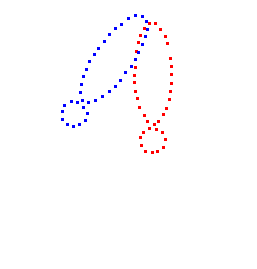
\includegraphics[width=0.30\textwidth]{LegRotation_Results_cropped}} 
		\\
		(a) & (b) & (c)
	\end{tabular}
	\caption{The joints $J_i$ and $J_j$ (green dots) of the reference cluster $C_i$ (red) and the target cluster $C_j$ (blue) are overlapped. The closest points for $C_i$ are computed (a). Stepwise rotation of $C_i$ onto $C_j$ in the direction of a decreasing error until $e$ does not further decrease (b). Final overlapping clusters from taking all closest points of $C_i$ and $C_j$ below a distance threshold $\tau$ (c).} 
	\label{fig:jointRotation}
\end{figure}
%%
With varying distance thresholds $\tau$ for the selection of closest points or region growing, actual target points may be skipped or unnecessary points from another rigid part are added. Those circumstances lead to difficulties for the detection of linked parts. Detailed results about this appearance is discussed in section \ref{ResultsLRP}.

\section{Implementation}
\label{ImplementationLRP}
For the implementation in Java the individual steps of the largest rigid part algorithm have been split into individual classes for a better overview. Again ImageJ was used as processing library.
%
%TODO: Add class graph of implementation
%

\subsection{Iterative Segmentation}
The whole algorithm initiates from the \texttt{Segmentation} class, where all steps proposed in section \ref{LRP} are implemented (see algorithm \ref{alg:segmentation}). Basically, the segmentation proceeds until no unclustered points from $C_1$ and $C_2$ are remaining. As a first step of the iterative segmentation approach already detected rigid parts are removed from the unclustered points (\texttt{removeAllLRPs()}). As a next step, clusters are detected either for an initial input or in case of an already detected LRP, to detect its the linked parts. Joints are only estimated in case of a previously detected rigid part which is the case for all iterations except the first one. Then, all matching clusters are added to a \texttt{Stack} (\texttt{pushMatchingClusters()}) to be processed in form of a ``last in - first out'' procedure. In case of an empty stack, all clusters have been processed and the algorithm terminates. 

\begin{lstlisting}
while (unclusteredReference.size() > MIN_SIZE || !clusters.isEmpty()) {

	removeAllLRPs();

	referenceClusters = RegionGrowing.detectClusters(unclusteredReference);
	targetClusters = RegionGrowing.detectClusters(unclusteredTarget);

	if (currentLrps != null) {
		detectJoints(currentLrps, referenceClusters, targetClusters);
	}

	if (referenceClusters.size() != 0 && targetClusters.size() != 0) {
		pushMatchingClusters();
	}

	if (clusters.isEmpty()) {
		return;
	}
...
}
\end{lstlisting}

If there are still clusters existent, two matching ones are popped from the Stack. If the clusters do not own an allocated joint, no LRP has been detected yet. Therefore, the \texttt{FeatureMatching} class (see subsection \ref{FeatureMatching}) is applied on the matching clusters. In combination with RANSAC a largest rigid part can be detected. On the other hand two LRPs can be detected by rotation two clusters around their joints. In this case the \texttt{PartDetection} class is taken advantage of to detect a linked rigid part to the previously detected LRP.

\begin{lstlisting}
while (unclusteredReference.size() > MIN_SIZE || !clusters.isEmpty()) {
...
	currentClusters = clusters.pop();

	if (currentClusters[0].getJoint() == null) {
		FeatureMatching fm = new FeatureMatching(currentClusters[0], currentClusters[1]);
		Map<Integer, Integer> denseCorrespondances = fm.getCorrespondences();

		if (denseCorrespondances.size() < 3) {
		return;
		}

		RANSAC ransac = new RANSAC(currentClusters[0], currentClusters[1], denseCorrespondances);
		currentLrps = ransac.getLargestRigidParts();
		unclusteredReference = ransac.getTransformedReferencePoints();
	}

	else {
		PartDetection pd = new PartDetection(currentClusters[0], currentClusters[1]);
		currentLrps = pd.getLinkedParts();
	}

	if (currentLrps[0].getPoints().size() < 5) {
	} else {
	largestRigidParts.add(currentLrps);
	}
}
\end{lstlisting}
%%
%TODO: Write algorithm for Segmentation
%%
\begin{algorithm}[tbp]
	\caption{Computation of the normal and subsequently feature histograms of a cluster point $p_i$ with its $k$ neighbors inside a radius $r$. The fast point feature histograms FPFH are computed by weighting the SPFH of a $p_i$ and its $k$ neighbors.}
	
	\begin{algorithmic}[1]     % [1] = all lines are numbered
		\label{alg:segmentation}
		
		\Procedure{FPFH}{$p_i$} 
		\State $\mathit{C_{max}} \gets ()$
		\State $\mathit{C_{current}} \gets ()$
		\State $n \gets \mathit{sizeOf}(M)$
		\State $m \gets \mathit{sizeOf}(C_{current})$
		
		\While {$n$ > 0}
		\State $\mathit{c_{current}} \gets \mathit{c_{current}} + \boldsymbol{u}_1$
		\For{$i = 1,\ldots,m$}
		\State $M \gets M - C_{current}$
		\For{$j = 1,\ldots,n$}
		\If {\Call{$d$}{$\boldsymbol{p}_i, \boldsymbol{u}_j}< \tau$}
		\State $C_{current} \gets C_{current} + \boldsymbol{u}_j$
		\EndIf
		\EndFor
		\EndFor
		\State $M \gets M - C_{current}$
		\If{$m > \mathit{sizeOf}(C_{max})$}
		\State $C_{max} \gets C_{current}$
		\EndIf
		\State $C_{current} \gets ()$
		\EndWhile
		\State\Return $C_{max}$
		\EndProcedure	
	\end{algorithmic}
\end{algorithm}

\subsection{Feature Matching}
\label{FeatureMatching}
For the computation of normals, required for the computation of feature histograms, the class \texttt{NormalEstimation} is developed. It takes a point $p_i$ with its $m$ neighbors as input. Then, the least fitting error line on those input points is detected (as described in section \ref{correspondences}) and the smallest lambda value $\lambda_2$ selected as eigenvalue. By setting the x-value of the normal to 1.0, the y-value can be calculated with the eigenvalue $\lambda_2$. The resulting vector represents the normal vector $\vec{n}$ for $p_i$. In case of being exactly vertically or horizontally, the resulting value for y is either $infinite$ or $NaN$. In these cases the normal is either set to (0,1) or (1,0). As a last step, the normal is normalized.
%%
\begin{lstlisting}
double eigenvalue = Math.min(lambda1, lambda2);

	covarianceMatrix = new double[][] { 
		{ a - eigenvalue, b},
		{ b, c - eigenvalue}
	};

	double[] normal = new double[2];

	normal[0] = 1.0;
	normal[1] = (eigenvalue * normal[0] - covarianceMatrix[0][0] * normal[0])/covarianceMatrix[0][1];

	if(Double.isInfinite(normal[1])){
		normal[0] = 0;
		normal[1] = 1;
	} else if (Double.isNaN(normal[1])){
		normal[1] = 0;
	}

double length = Math.sqrt(Math.pow(normal[0], 2) + Math.pow(normal[1], 2));
normal[0] /= length;
normal[1] /= length;

point.setNormal(normal);
\end{lstlisting}
%%
A \texttt{ClusterPoint} class was implemented to store the normal $n_i$ for each point and the resulting feature histogram (FPFH) in form of a \texttt{Histogram} object containing an \texttt{int[]} array. For the calculation of a feature histogram of a point $p_i$, its $k$ neighbors are taken into account. The \texttt{FPFH} class implements various operations for vectors, like a dot or cross product to implement the formula from subsection \ref{FPFH}.
%%
\begin{lstlisting}
public void featureHistogram(p_i) {
	SPFH = SPFH(p_i);

	for (ClusterPoint p_k : p_i.getNeighborhood()) {
		double weight = p_i.distance(p_k);
		weightedSPFH = weightedSPFH.addHistograms(SPFH(p_k).multiplyHistograms(1.0 / weight));
	}
	
	FPFH = SPFH.addHistograms(weightedSPFH.multiplyHistograms(1.0 / p_i.getNeighborhood().size()));
	
	p_i.setFPFH(FPFH);
}
\end{lstlisting}

%TODO implementation of FPFH (index)

The feature histogram is computed by calculating the SPFH of a point by calculating angles between all its neighbors.



The combination of those three angles leads to an index in the histogram to be incremented. 





%%
Subsequently, point correspondences are detected by computing the distances between all feature histograms of $C_1$ and $C_2$ (see section \ref{correspondences}). For that, the closest point algorithm is configured to use the distance between histograms instead of the euclidean distance of point locations. Reciprocal point correspondences between $C_1$ and $C_2$ are returned in form of point indices \texttt{Map<Integer,Integer>}  of the clusters cluster points.
%%
%TODO: show chi-square distance
%%
\begin{lstlisting}
for (Map.Entry<Integer, Integer> entry : reference.entrySet()) {
	Integer referenceIndex = entry.getKey();
	Integer targetIndex = entry.getValue();

	ClusterPoint currentRefPoint = originalReference.get(referenceIndex);
	ClusterPoint currentTargetPoint = originalTarget.get(targetIndex);
...
	if ((reciprocalMatching && target.get(targetIndex) == referenceIndex){
		finalReferencePoints.add(currentRefPoint);
		finalTargetPoints.add(currentTargetPoint);
		finalAssociations.put(referenceIndex, targetIndex);
	}
}
\end{lstlisting}
%%
%TODO: add algorithm of FPFH + normals
%%
\begin{algorithm}[tbp]
	\caption{Computation of the normal and subsequently feature histograms of a cluster point $p$ with its $k$ neighbors inside a radius $r$. The fast point feature histograms FPFH are computed by weighting the SPFH of a $p_i$ and its $k$ neighbors.}
	
	\begin{algorithmic}[1]     % [1] = all lines are numbered
		\label{featureHistograms}
		
		\Procedure{FPFH}{$p_i$} 
		\State $\mathit{C_{max}} \gets ()$
		\State $\mathit{C_{current}} \gets ()$
		\State $n \gets \mathit{sizeOf}(M)$
		\State $m \gets \mathit{sizeOf}(C_{current})$
		
		\While {$n$ > 0}
		\State $\mathit{c_{current}} \gets \mathit{c_{current}} + \boldsymbol{u}_1$
		\For{$i = 1,\ldots,m$}
		\State $M \gets M - C_{current}$
		\For{$j = 1,\ldots,n$}
		\If {\Call{$d$}{$\boldsymbol{p}_i, \boldsymbol{u}_j}< \tau$}
		\State $C_{current} \gets C_{current} + \boldsymbol{u}_j$
		\EndIf
		\EndFor
		\EndFor
		\State $M \gets M - C_{current}$
		\If{$m > \mathit{sizeOf}(C_{max})$}
		\State $C_{max} \gets C_{current}$
		\EndIf
		\State $C_{current} \gets ()$
		\EndWhile
		\State\Return $C_{max}$
		\EndProcedure	
	\end{algorithmic}
\end{algorithm}
%%
%TODO: add code snippet of feature calculation

\subsection{RANSAC}
\label{RANSAC}
The RANSAC algorithm takes the computed dense correspondences between two clusters in form of a \texttt{Map<Integer, Integer>} as input. As a first step, two random correspondences are selected from the map to calculate an affine transformation between the three resulting points from each $C_i$ and $C_j$. The initial orientation and alignment is thereby irrelevant as the transformation $T$ is completely recalculated.
%%
\begin{lstlisting}
public LargestRigidPart(Cluster c_i, Cluster c_j, Map<Integer, Integer> correspondences)
...
points1 = c_i.getPoints();
points2 = c_j.getPoints();
...
private void getRandomPoints(int num) {
	Integer[] keys = correspondances.keySet().toArray(new Integer[0]);
	Integer[] values = correspondances.values().toArray(new Integer[0]);

	for (int i = 0; i < num; i++) {
		index = (int) (Math.random() * correspondances.size());
		randomPoints1.add(points1.get(keys[index]));
		randomPoints2.add(points2.get(values[index]));
	}
}
...
\end{lstlisting}
%%
In each iteration a region growing approach with a threshold $\tau$ is conducted on all overlapping points. The value is thereby considerably small as a right alignment during any iteration is assumed. The biggest cluster is stored and after termination of the procedure returned as largest rigid part. The whole RANSAC approach is considerable time consuming. It can be reduced by taking a smaller number of correspondences as input which directly affects the required number of iterations until a right match is detected (see section \ref{ResultsLRP}).

\subsection{Joint rotation}
The main part for the detection of linked parts from clusters grown from already detected LRP is the rotation around their estimated joints. As a first step, both clusters are moved to the origin and are similarly aligned.
%%
\begin{lstlisting}
if (c_i.getJoint() != null) {
	referencePoints = Matrix.translate(c_i.getPoints(), -c_i.getJoint().getX(), -c_i.getJoint().getY());
	targetPoints = Matrix.translate(c_j.getPoints(), -c_j.getJoint().getX(), -c_j.getJoint().getY());
	initialOrientation(c_i.getJoint());
	}
\end{lstlisting}
%%
As a next step, the reference points are aimed to be rotated onto the target points. This is achieved iteratively by applying a rotation in the direction of an achieved reduced error. By computing an error for each iteration, the assumed biggest overlap is achieved.
%%
\begin{lstlisting}
for (Map.Entry<Integer, Integer> entry : correspondences.entrySet()) {
...
	totalError += currentError / referencePoint.distance(new ClusterPoint(0,0));	
...	
}
\end{lstlisting}
%%
To only remain the rigid part and reject corresponding points that do not belong to the searched part, a region growing algorithm is applied. As a result only the largest cluster as successful detected rigid part is kept (see subsection \ref{RegionGrowing}).

\section{Results}
\label{ResultsLRP}

Applying the proposed approach on the 2D data set of an articulated object, following results could be achieved with adjusted parameters based on the estimated resolutions of 7.24 and 7.56. (see Table \ref{table:parameters}).

\begin{itemize}
	\item[RG] Region Growing for Noise removal
	\item[LRP] Region growing for largest rigid part
	\item[CPPC] Closest point for part detection 
	\item[RGPC]	Region growing for part detection
	\item[DC] distance criteria for feature matching
\end{itemize}

\begin{table}
	\centering
	\begin{tabular}{ |c|c|c|c|c| } 
		\hline
		Iteration & $\tau$ RG  & $\tau$ CPPD & $\tau$ LRP & DC \\
		\hline
		1& 3 & 21 & 14 & Euclidean \\ 
		2& 5 & 3 & 2 & Euclidean \\
		3& 7 & 2 & 2 & Euclidean\\
		4& 4 & 38 & 31 & Euclidean \\ 
		5& 6 & 4 & 3 & Euclidean\\
		& 8 & 3 & 3 & Euclidean\\
		& 6 & 35 & 26 & Euclidean\\ 
		4 & 7 & 3 & 3 & Euclidean \\
		& 8 & 3 & 3 & Euclidean \\
		\hline
	\end{tabular}
	\caption{Segmentation results}
	\label{table:parameters}
\end{table}

Unfortunately, not all rigid parts as well as joints could be detected right using following parameters: 

\begin{figure}[H]
	\centering\small
	\begin{tabular}{cc}
		\fbox{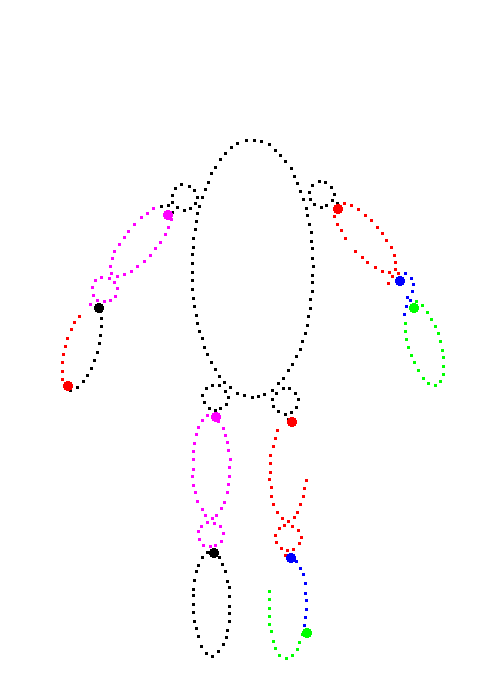
\includegraphics[width=0.40\textwidth]{results/final/final1_12-rgTH_4-JointTH_3-RansacTH_ED}} &	
		\fbox{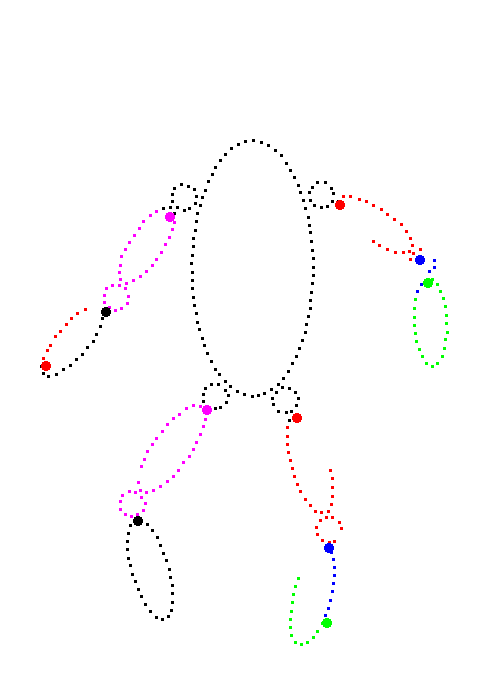
\includegraphics[width=0.40\textwidth]{results/final/final2_12-rgTH_4-JointTH_3-RansacTH_ED}} 
		\\
		(a) & (b) 
	\end{tabular}
	\caption{Initial results with standard parameters estimated from the resolution from $C_1$ (a) and $C_2$ (b).} 
	\label{fig:initialResults}
\end{figure}

Improved results could be achieved by adjusting different parameters, like the number $k$ of nearest neighbors considered for the computation of normals and features. Furthermore, different histogram similarity criteria are applied for the feature matching (see subsection \ref{HistogramSimilarity}). 

\begin{figure}[H]
	\centering\small
	\begin{tabular}{cc}
		\fbox{
\includegraphics[width=0.40\textwidth]{Placeholder}} &	
		\fbox{
\includegraphics[width=0.40\textwidth]{Placeholder}} 
		\\
		(a) & (b) 
	\end{tabular}
	\caption{Initial results with standard parameters estimated from the resolution from $C_1$ (a) and $C_2$ (b).} 
	\label{fig:initialResults}
\end{figure}

\begin{figure}[H]
	\centering\small
	\begin{tabular}{cc}
		\fbox{
\includegraphics[width=0.40\textwidth]{Placeholder}} &	
		\fbox{
\includegraphics[width=0.40\textwidth]{Placeholder}} 
		\\
		(a) & (b) 
	\end{tabular}
	\caption{Initial results with standard parameters estimated from the resolution from $C_1$ (a) and $C_2$ (b).} 
	\label{fig:initialResults}
\end{figure}

%TODO: add alternate pictures of LRP results

\subsection{Histogram distances for feature matching}
\label{HistogramSimilarity}

As histogram similarity criteria three different distances are considered: the euclidean, the chi-square and the Kullback-Leibler distance (see figure \ref{fig:histogramCriteria}). The euclidean distance results in the highest number of point correspondences compared to the other two histogram distances. This results in a higher number of RANSAC iterations as more wrong point correspondences are present. On the other hand also the number of correct correspondences is higher. Thus, the overall probability of detecting the LRP is considerable high. In case of applying the chi-square distance, less correspondences are detected. But in contrary to the euclidean distance, a higher ratio of right correspondences is achieved. This leads to a lower number of RANSAC iterations, which supports the goal of a less computation-expensive segmentation approach. Finally, the Kullback-Leibler distance detects only a few correspondences, including only a considerable small ratio of correct correspondences. As a consequence, the LRP might not be detected during the RANSAC iterations which denotes this distance as not useful for this approach.

\begin{figure}[H]
	\centering\small
	\begin{tabular}{ccc}
		\fbox{
\includegraphics[width=0.23\textwidth]{Placeholder}} &	
		\fbox{
\includegraphics[width=0.23\textwidth]{Placeholder}} &		
		\fbox{
\includegraphics[width=0.23\textwidth]{Placeholder}} 
		\\
		(a) & (b) & (c)
	\end{tabular}
	\caption{Applying different histogram distances on the feature histograms of $C_1$ and $C_2$ in order to detect point correspondences. The euclidean distance(a), the chi-square distance(b) and the Kullback-Leibler distance(c) are contrasted.} 
	\label{fig:histogramCriteria}
\end{figure}

In terms of runtime, the euclidean distance represents the fastest choice, followed by the chi-squared and the Kullback-Leibler. 

%TODO: RUNTIME!

\subsection{Main drawbacks}
The main drawback of the algorithm represents the first initial alignment of $C_1$ and $C_2$ to detect the actual largest rigid part of the articulated object. In case of a failure, the linked rigid parts can not be detected as they are directly dependent a successful initial alignment. By increasing the number of RANSAC iterations, the probability of a correct initial alignment can be increased, however this directly affects the runtime and should therefore not be exaggerated. A major factor for the successful detection of a LRP poses the input data in form a point cloud. As the object's surface is imitated by the objects'hull composed of 2D points the region growing is much more error-prone. The reason is, that unlike as in 3D, the points of a rigid part in 2D have a considerable lower number of neighbors. In case of a few missing cluster points from a rigid part, it will not be fully detected during the region growing due to the resulting offset. This is especially drastically during the RANSAC approach as it results in the initial LRP. To counteract this behavior, more and closer hull points can be added to each rigid part. A further main problem is that the algorithm proceeds iteratively from already detected rigid parts. This makes the whole procedure notable unstable and error prone, as one faulty rigid part detection leads to an overall unsuccessful segmentation of an articulated object. Furthermore, touching of rigid parts (e.g. the hand touches the leg) would constitute difficulties as the region growing would detect those as potential linked clusters. Most of the discussed drawbacks concerning the input data can be overcome by an implementation in 3D (see section \ref{3DImplementation}). 

\section{3D implementation}
\label{3DImplementation}
The next step would be to transfer the optimized 2D implementation into 3D to reduce the computation steps from \cite{guo2016correspondence} (see section \ref{functionalityLRP}). It can be implemented by using the Point Cloud library \footnote{http://pointclouds.org} which operates with 3D point clouds. Certainly, many new challenges will have to be overcome due to the three-dimensional space. The straightforward rotation from linked rigid parts around their estimated joints will pose a major difficulty in 3D as multiple rotation axes are available. On the other hand it is noticeable that PCL offers many required functions by default. For example, the Fast Point Feature Histogram completed with the normal estimation as well as sub sampling of dense point clouds are already provided. 

%TODO: add code snippet of PCL


An appropriate dataset as input constitutes the SCAPE data set which provides different poses of a human (see figure \ref{fig:SCAPE}).

%TODO: add reference of SCAPE data

\begin{figure}[H]
	\centering\small
	\begin{tabular}{cc}
		\fbox{
\includegraphics[width=0.23\textwidth]{Placeholder}} &			
		\fbox{
\includegraphics[width=0.23\textwidth]{Placeholder}} 
		\\
		(a) & (b)
	\end{tabular}
	\caption{Taking two 3D poses of an articulated object as input, the segmentation approach can be shifted to 3D.} 
	\label{fig:SCAPE}
\end{figure}

